%%
%% Automatically generated file from DocOnce source
%% (https://github.com/hplgit/doconce/)
%%

% #define PREAMBLE

% #ifdef PREAMBLE
%-------------------- begin preamble ----------------------

\documentclass[%
oneside,                 % oneside: electronic viewing, twoside: printing
final,                   % draft: marks overfull hboxes, figures with paths
10pt]{article}

\listfiles               %  print all files needed to compile this document

\usepackage{relsize,makeidx,color,setspace,amsmath,amsfonts,amssymb}
\usepackage[table]{xcolor}
\usepackage{bm,ltablex,microtype}

\usepackage[pdftex]{graphicx}

% Packages for typesetting blocks of computer code
\usepackage{fancyvrb,framed,moreverb}

% Define colors
\definecolor{orange}{cmyk}{0,0.4,0.8,0.2}
\definecolor{tucorange}{rgb}{1.0,0.64,0}
\definecolor{darkorange}{rgb}{.71,0.21,0.01}
\definecolor{darkgreen}{rgb}{.12,.54,.11}
\definecolor{myteal}{rgb}{.26, .44, .56}
\definecolor{gray}{gray}{0.45}
\definecolor{mediumgray}{gray}{.8}
\definecolor{lightgray}{gray}{.95}
\definecolor{brown}{rgb}{0.54,0.27,0.07}
\definecolor{purple}{rgb}{0.5,0.0,0.5}
\definecolor{darkgray}{gray}{0.25}
\definecolor{darkblue}{rgb}{0,0.08,0.45}
\definecolor{darkblue2}{rgb}{0,0,0.8}
\definecolor{lightred}{rgb}{1.0,0.39,0.28}
\definecolor{lightgreen}{rgb}{0.48,0.99,0.0}
\definecolor{lightblue}{rgb}{0.53,0.81,0.92}
\definecolor{lightblue2}{rgb}{0.3,0.3,1.0}
\definecolor{lightpurple}{rgb}{0.87,0.63,0.87}
\definecolor{lightcyan}{rgb}{0.5,1.0,0.83}

\colorlet{comment_green}{green!50!black}
\colorlet{string_red}{red!60!black}
\colorlet{keyword_pink}{magenta!70!black}
\colorlet{indendifier_green}{green!70!white}

% Backgrounds for code
\definecolor{cbg_gray}{rgb}{.95, .95, .95}
\definecolor{bar_gray}{rgb}{.92, .92, .92}

\definecolor{cbg_yellowgray}{rgb}{.95, .95, .85}
\definecolor{bar_yellowgray}{rgb}{.95, .95, .65}

\colorlet{cbg_yellow2}{yellow!10}
\colorlet{bar_yellow2}{yellow!20}

\definecolor{cbg_yellow1}{rgb}{.98, .98, 0.8}
\definecolor{bar_yellow1}{rgb}{.98, .98, 0.4}

\definecolor{cbg_red1}{rgb}{1, 0.85, 0.85}
\definecolor{bar_red1}{rgb}{1, 0.75, 0.85}

\definecolor{cbg_blue1}{rgb}{0.87843, 0.95686, 1.0}
\definecolor{bar_blue1}{rgb}{0.7,     0.95686, 1}

%\setlength{\fboxsep}{-1.5mm}  % adjust cod_vpad/pro_vpad background box

%% Background for code blocks (parameter is color name)

%% pro/cod_vpad: gives some vertical padding before and after the text
%% (but has more simplistic code than _cod/pro_tight+cod/pro).
%% pro/cod_vpad can be used to enclose Verbatim or lst begin/end for code.
%% pro/cod calls _pro/cod_tight and has very little vertical padding,
%% used to enclose Verbatim and other begin/end for code.
%% (pro/cod is what the ptex2tex program could produce with the
%% Blue/BlueBar definitions in .ptex2tex.cfg.)

\newenvironment{cod_vpad}[1]{
   \def\FrameCommand{\colorbox{#1}}
   \MakeFramed{\FrameRestore}}
   {\endMakeFramed}

\newenvironment{_cod_tight}[1]{
   \def\FrameCommand{\colorbox{#1}}
   \FrameRule0.6pt\MakeFramed {\FrameRestore}\vskip3mm}
   {\vskip0mm\endMakeFramed}

\newenvironment{cod}[1]{
\bgroup\rmfamily
\fboxsep=0mm\relax
\begin{_cod_tight}{#1}
\list{}{\parsep=-2mm\parskip=0mm\topsep=0pt\leftmargin=2mm
\rightmargin=2\leftmargin\leftmargin=4pt\relax}
\item\relax}
{\endlist\end{_cod_tight}\egroup}

%% Background for complete program blocks (parameter 1 is color name
%% for background, parameter 2 is color for left bar)
\newenvironment{pro_vpad}[2]{
   \def\FrameCommand{\color{#2}\vrule width 1mm\normalcolor\colorbox{#1}}
   \MakeFramed{\FrameRestore}}
   {\endMakeFramed}

\newenvironment{_pro_tight}[2]{
   \def\FrameCommand{\color{#2}\vrule width 1mm\normalcolor\colorbox{#1}}
   \FrameRule0.6pt\MakeFramed {\advance\hsize-2mm\FrameRestore}\vskip3mm}
   {\vskip0mm\endMakeFramed}

\newenvironment{pro}[2]{
\bgroup\rmfamily
\fboxsep=0mm\relax
\begin{_pro_tight}{#1}{#2}
\list{}{\parsep=-2mm\parskip=0mm\topsep=0pt\leftmargin=2mm
\rightmargin=2\leftmargin\leftmargin=4pt\relax}
\item\relax}
{\endlist\end{_pro_tight}\egroup}

\usepackage{minted}
\usemintedstyle{default}

\usepackage[T1]{fontenc}
%\usepackage[latin1]{inputenc}
\usepackage{ucs}
\usepackage[utf8x]{inputenc}

\usepackage{lmodern}         % Latin Modern fonts derived from Computer Modern

% Hyperlinks in PDF:
\definecolor{linkcolor}{rgb}{0,0,0.4}
\usepackage{hyperref}
\hypersetup{
    breaklinks=true,
    colorlinks=true,
    linkcolor=linkcolor,
    urlcolor=linkcolor,
    citecolor=black,
    filecolor=black,
    %filecolor=blue,
    pdfmenubar=true,
    pdftoolbar=true,
    bookmarksdepth=3   % Uncomment (and tweak) for PDF bookmarks with more levels than the TOC
    }
%\hyperbaseurl{}   % hyperlinks are relative to this root

\setcounter{tocdepth}{2}  % levels in table of contents

% Tricks for having figures close to where they are defined:
% 1. define less restrictive rules for where to put figures
\setcounter{topnumber}{2}
\setcounter{bottomnumber}{2}
\setcounter{totalnumber}{4}
\renewcommand{\topfraction}{0.95}
\renewcommand{\bottomfraction}{0.95}
\renewcommand{\textfraction}{0}
\renewcommand{\floatpagefraction}{0.75}
% floatpagefraction must always be less than topfraction!
% 2. ensure all figures are flushed before next section
\usepackage[section]{placeins}
% 3. enable begin{figure}[H] (often leads to ugly pagebreaks)
%\usepackage{float}\restylefloat{figure}

% --- fancyhdr package for fancy headers ---
\usepackage{fancyhdr}
\fancyhf{} % sets both header and footer to nothing
\renewcommand{\headrulewidth}{0pt}
\fancyfoot[LE,RO]{\thepage}
% Ensure copyright on titlepage (article style) and chapter pages (book style)
\fancypagestyle{plain}{
  \fancyhf{}
  \fancyfoot[C]{{\footnotesize \copyright\ 2021, Ahmed Ammar. Released under CC Attribution 4.0 license}}
%  \renewcommand{\footrulewidth}{0mm}
  \renewcommand{\headrulewidth}{0mm}
}
% Ensure copyright on titlepages with \thispagestyle{empty}
\fancypagestyle{empty}{
  \fancyhf{}
  \fancyfoot[C]{{\footnotesize \copyright\ 2021, Ahmed Ammar. Released under CC Attribution 4.0 license}}
  \renewcommand{\footrulewidth}{0mm}
  \renewcommand{\headrulewidth}{0mm}
}

\pagestyle{fancy}


% prevent orhpans and widows
\clubpenalty = 10000
\widowpenalty = 10000

% --- end of standard preamble for documents ---


% insert custom LaTeX commands...

\raggedbottom
\makeindex
\usepackage[totoc]{idxlayout}   % for index in the toc
\usepackage[nottoc]{tocbibind}  % for references/bibliography in the toc

%-------------------- end preamble ----------------------

\begin{document}

% matching end for #ifdef PREAMBLE
% #endif

\newcommand{\exercisesection}[1]{\subsection*{#1}}


% ------------------- main content ----------------------



% ----------------- title -------------------------

\thispagestyle{empty}

\begin{center}
{\LARGE\bf
\begin{spacing}{1.25}
Équations différentielles ordinaires
\end{spacing}
}
\end{center}

% ----------------- author(s) -------------------------

\begin{center}
{\bf Ahmed Ammar (\texttt{ahmed.ammar@fst.utm.tn})}
\end{center}

    \begin{center}
% List of all institutions:
\centerline{{\small Institut Préparatoire aux Études Scientifiques et Techniques, Université de Carthage.}}
\end{center}
    
% ----------------- end author(s) -------------------------

% --- begin date ---
\begin{center}
Jan 13, 2021
\end{center}
% --- end date ---

\vspace{1cm}


\tableofcontents


\vspace{1cm} % after toc




\section{Introduction}
Dans les domaines scientifiques et industriels, il est courant aujourd'hui d'étudier la nature ou les dispositifs technologiques au moyen de modèles sur ordinateur. Avec de tels modèles, l'ordinateur agit comme un laboratoire virtuel où les expériences peuvent être effectuées de manière rapide, fiable, sûre et économique.

Les équations différentielles constituent l'un des outils mathématiques les plus puissants pour comprendre et prédire le comportement des systèmes dynamiques de la nature, de l'ingénierie et de la société. Un système dynamique est un système avec un état, généralement exprimé par un ensemble de variables, évoluant dans le temps. Par exemple, un pendule oscillant, la propagation d'une maladie et les conditions météorologiques sont des exemples de systèmes dynamiques. Nous pouvons utiliser les lois fondamentales de la physique, ou l'intuition simple, pour exprimer des règles mathématiques qui régissent l'évolution du système dans le temps. Ces règles prennent la forme d'équations différentielles.


\section{Loi de désintégration radioactive}

La radioactivité a été découverte en France, de 1896 à 1898, par Henri Becquerel, qui a mis en évidence l’existence d’un rayonnement invisible provenant de l’uranium (voir Figure~\ref{fig:Becquerel}), et par Pierre et Marie Curie qui ont montré la généralité de ce phénomène, lui ont donné son nom, et découvert deux éléments chimiques particulièrement radioactifs, le polonium et le radium. Dans l’histoire de cette découverte, et du développement de toutes ses conséquences, on retrouve toutes les grandes questions liées à la recherche, aux mécanismes de la découverte, aux remises en cause des acquis de la science et à l’exploitation scientifique, technologique et industrielle des connaissances nouvelles.


\begin{figure}[!ht]  % fig:Becquerel
  \centerline{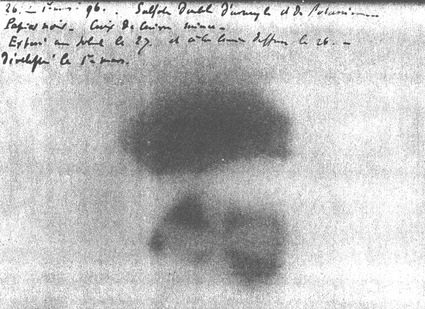
\includegraphics[width=0.7\linewidth]{imgs/radioactivite.jpg}}
  \caption{
  Cliché développé par Becquerel le $1^{er}$ mars 1896 après être resté dans un tiroir. On distingue dans la tache inférieure, une croix de Malte à laquelle Becquerel fait allusion (« Si, entre la lamelle du sel d’uranium et la lame d’aluminium ou le papier noir, on interpose un écran formé d’une lame de cuivre … par exemple en forme de croix, on observe dans l’image la silhouette de cette croix, en plus clair… »). Les annotations sont de la main de Becquerel.[s:OpenEdition Journals, \href{{https://journals.openedition.org/bibnum/848}}{Henri Becquerel : découverte de la radioactivité}] \label{fig:Becquerel}
  }
\end{figure}
%\clearpage % flush figures fig:Becquerel


On veut modéliser numériquement l’évolution d’un échantillon radioactif. On prendra les valeurs numériques du plutonium 238 , un isotope radioactif du plutonium ayant une constante radioactive $\lambda$ = 0,79 siècle$^{-1}$ qui se désintègre en émettant des particules $\alpha$.
On veut modéliser l’évolution temporelle d’un échantillon de plutonium 238 contenant initialement $N_0$ = $10^{23}$ atomes.

Par définition, la constante radioactive $\lambda$ est la probabilité qu’un atome se désintègre par unité de temps.

Si à l’instant $t$, l’échantillon contient $N(t)$ atomes, le nombre $dN$ d’atomes se désintégrant entre les instants $t$ et $t + dt$ est donc :
\begin{equation}
dN(t) = - \lambda N(t) \ dt
\label{eq:desintegration_ode}
\end{equation}
Cette équation peut être intégrée directement, avec la solution:
\begin{equation}
N(t) = N_0 e^{-\lambda t}
\label{eq:desintegration_exact}
\end{equation}
mais nous voulons essayer de résoudre l'équation numériquement.

L'approche la plus simple consiste à exprimer le nombre de noyaux à l'instant $t + \Delta t$ en termes de nombre à l'instant $t$:

\begin{equation}
N(t + \Delta t) = N(t) - \lambda N(t) \Delta t + \mathcal{O}(\Delta t^2)
\label{eq:desintegration_euler}
\end{equation}
Si nous commençons par $N_0$ noyaux à l'instant $t = 0$, alors à $t = \Delta t$ nous aurons $N(\Delta t) \approx N_0 - (\lambda N_0) \Delta t$; at $t = 2 \Delta t$ nous aurons $N(2\Delta t) \approx N(\Delta t) - [\lambda N(\Delta t)] \Delta t$ etc.
L'erreur de troncature est $\mathcal{O}(\Delta t^2)$. Par conséquent, si la taille du pas $\Delta t$ est petite, nous nous attendons à ce que notre solution numérique soit proche de la solution exacte. Cette méthode d’intégration d’une équation différentielle ordinaire est connue sous le nom de \textbf{méthode d’Euler}.



\vspace{6mm}

% inline figure
\centerline{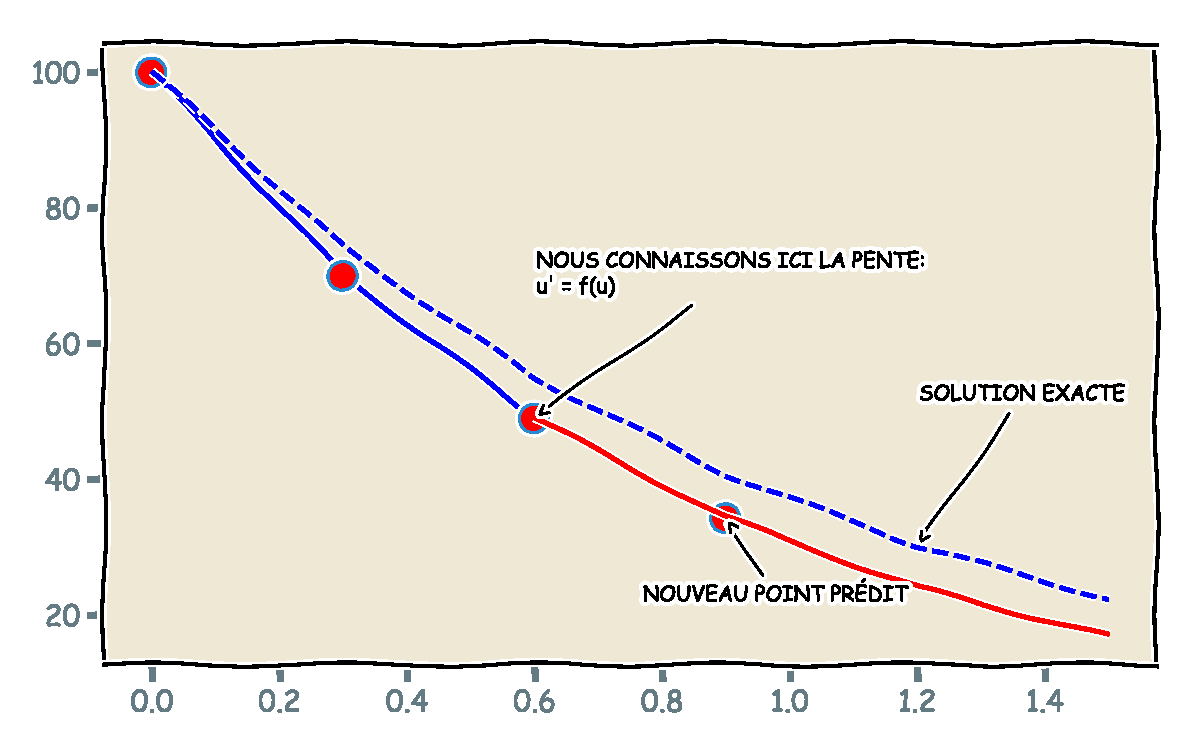
\includegraphics[width=0.7\linewidth]{scripts/euler_schema.pdf}}

\vspace{6mm}



Pour limiter les erreurs dues à l’implémentation de certains algorithmes ou à la précision limitée de la machine sur laquelle on travaille, on choisit souvent en physique numérique de travailler dans des systèmes d’unités adaptés, qui donnent des valeurs numériques raisonnables. On pourra ici exprimer les temps en siècles et les quantités de matières en moles (1 mol = 6,02 $\times 10^{23}$ entités élémentaires).

\begin{itemize}
\item \textbf{Q1.} Écrire une fonction \texttt{radioactivite} en Python prenant comme arguments un nombre initial d’atomes $N_0$ , une valeur maximale $t_max$ de $t$, un pas $\Delta t$ et une probabilité de désintégration $\lambda$ et qui retourne deux listes contenant les valeurs de $t_n$ et les valeurs de $N(t_n)$ correspondantes. La syntaxe pour retourner deux listes et les utiliser est la suivante :
\end{itemize}

\noindent
\begin{cod}{cbg_gray}\begin{minted}[fontsize=\fontsize{9pt}{9pt},linenos=false,mathescape,baselinestretch=1.0,fontfamily=tt,xleftmargin=2mm]{python}
def radioactvite (N0 , tmax , delta_t , Lambda ) :
    #Le code de la fonction qui crée deux listes liste_t et liste_N
    #...
    return liste_t, liste_N

l_t , l_N = radioactivite(N0 , tmax , delta_t , Lambda)
\end{minted}
\end{cod}
\noindent

\begin{itemize}
\item \textbf{Q2.} En utilisant matplotlib, tracer l’allure de $N(t)$ obtenue pour quelques valeurs de $\Delta t$ (0,01 siècle, 0,1 siècle et 1 siècle, par exemple), on pourra prendre $t_max$ = 5 siècles.

\item \textbf{Q3.} Tracer sur le même graphe que précédemment la solution exacte du problème Eq.(\ref{eq:desintegration_exact}). Quelle est l’influence de la valeur de $\Delta_t$ sur la qualité du résultat ?
% @@@CODE scripts/desintegration.py
% Le programme demande le nombre initial de noyaux, $N_0$, la constante de temps de décroissance $\tau$, le pas de temps $\Delta t$ et la durée totale de l'intégration $t_{max}$. Lorsque ce programme est exécuté avec les valeurs d'entrée sont; $N_0 = 100$, $\tau = 1$, $\Delta t = 0.04$ et $t_{max} = 5$, le programme produit le tracé présenté dans la Figure~\ref{figout:desintegration}.
% 
% FIGURE:[scripts/desintegration, width=500 frac=0.7] Résultat de l'exécution du programme \emph{desintegration.py} avec entrée $N_0 = 100$, $\tau = 1$, $\Delta t = 0.04$ et $t_{max} = 5$. \label{figout:desintegration}
% Voyons maintenant à quel point notre programme est proche de la solution exacte. Vraisemblablement, lorsque le pas $\Delta t$ est grand, l'erreur sera pire; aussi, les erreurs grandissent avec le temps. Pour voir cela, considérons une version modifiée de notre programme \emph{desintegration.py} qui trace la différence fractionnaire entre le résultat numérique et le résultat exact donné par Eq.~(\ref{eq:desintegration_exact}). Notre nouveau programme effectuera des évolutions numériques sur un certain nombre de \textbf{différentes valeurs du pas} afin que nous puissions voir comment l'erreur dépend du degré de raffinement de $\Delta t$.
% 
% @@@CODE scripts/desintegrationErr.py
% 
% Ce programme produit les résultats montrés à la Figure~\ref{figout:desintegrationErr}.
% 
% FIGURE:[scripts/desintegrationErr, width=500 frac=0.7] Résultat de l'exécution du programme \emph{desintegrationErr.py} avec entrée $N_0 = 100$, $\tau = 1$, $\Delta t = 0.1$, $N_{res}=4$ et $t_{max} = 10$. \label{figout:desintegrationErr}
% 
% Les erreurs se rapprochent de manière linéaire avec le temps (les lignes du tracé logarithmique ont une pente approximativement égale à l'unité) et chaque facteur de 10 dans le raffinement diminue l'erreur fractionnaire d'un facteur 10. Pour comprendre cela, notez que le terme que nous avons jeté dans l'expansion de Taylor de notre équation différentielle ordinaire était le terme $d^2 N / d t^2 $, donc chaque étape introduit une erreur de:
% !bt
% \begin{equation}
% e_i \approx \frac{1}{2} \frac{d^2 N(t_i)}{d t^2} \Delta t^2 = \frac{N(t_i)}{2 \tau^2} \Delta t^2
% \label{eq:local_erreur}
% \end{equation}
% % Ceci est connu sous le nom \textbf{d'erreur locale}. Si l'erreur locale d'un schéma d'intégration numérique est $\mathcal{O}(\Delta t^{p + 1})$ comme $t \rightarrow 0$, alors on dit que c'est l'ordre $p$. La méthode d’Euler est donc un schéma d’intégration de premier ordre. \textbf{L'erreur globale} est l'erreur accumulée lorsque l'intégration est effectuée pendant une certaine durée T. Le nombre d'étapes requis est $n = T / \Delta t$ et chaque étape $i~=~1...n$ accumule une erreur $e_i$, nous nous attendons donc à ce que l'erreur globale soit:
% !bt
% \begin{equation}
% E_n \le \sum_{i=1}^n e_i \le T \frac{N_0}{2 \tau^2} \Delta t
% \label{eq:global_erreur}
% \end{equation}
% % puisque $e_i \le \frac{N_0}{2 \tau^2} \Delta t^2$. Notez que pour un schéma d’intégration d'ordre $p$, l'erreur sera $\mathcal{O}(\Delta t^{p})$; de plus, l'erreur grandit avec le temps $T$. Pour la méthode d'Euler, l'erreur croît de manière approximativement linéaire avec $T$ et avec $\Delta t$, ce qui est ce que nous voyons sur la Figure~\ref{figout:desintegrationErr}.
% 
% !bnotice
% La méthode d'Euler n'est pas une méthode recommandée pour résoudre des équations différentielles ordinaires. S'agissant simplement du premier ordre, une précision souhaitée n'est obtenue que pour de très petites valeurs de $\Delta t$, de nombreuses étapes d'intégration sont donc nécessaires pour faire évoluer le système pour une durée donnée $T$. Mais le coût en calcul de la méthode d’Euler n’est pas son seul inconvénient: elle n’est pas particulièrement stable non plus, comme nous le verrons plus loin dans ce chapitre..
% !enotice
% 
% 
% ======= Mouvement d'un projectile =======
% Un autre exemple d'équation différentielle ordinaire est celui du mouvement du projectile, pour lequel les équations du mouvement sont:
% !bt
% \begin{align}
% \frac{dx}{dt} &=v_x, & \frac{dv_x}{dt} &=0, \\
% \frac{dy}{dt} &=v_y, & \frac{dv_y}{dt} &=-g,
% \end{align}
% % où $g$ est l'accélération de pesanteur. Nous pouvons utiliser la méthode d'Euler pour écrire chaque dérivée sous une forme de différence finie convenant à l'intégration numérique:
% 
% !bt
% \begin{align}
% x_{i+1} &  =x_i + v_{x,i} \Delta t, &  v_{x,i+1} &= v_{x,i}, \\
% y_{i+1} &  =y_i + v_{y,i} \Delta t, &  v_{y,i+1} &= v_{y,i} - g \Delta t,
% \end{align}
% % Les trajectoires d'un projectile lancé avec une vitesse $v_0~=~10~ \ m~s^{-1}$ à différents angles sont tracées par le programme \texttt{projectile.py} et sont tracées à la Fig.~\ref{fig:projectile}.
% @@@CODE scripts/projectile.py
% Nous voyons, comme prévu, que la plus grande plage est atteinte pour un angle de lancement de $45^\circ$.
% 
% FIGURE:[scripts/projectile, width=500 frac=0.7] Résultats de l'exécution du programme \texttt{projectile.py}. On voit que la plus grande plage est atteinte avec un angle de lancement de $\theta = 45^\circ$. \label{fig:projectile}
% 
% Trouver la trajectoire d'un projectile compte tenu de ses conditions initiales, $v_{x,i}$ et $v_{x,i}$ ou de manière équivalente $v_0$ et $\theta$, est relativement simple. Cependant, supposons que nous voulons trouver l'angle de lancement $\theta$ requis pour atteindre une cible à une distance donnée avec une vitesse initiale $v_0$ donnée. Ceci est un exemple de problème de la \emph{valeur aux limites} à deux points.Une approche pour résoudre un tel problème est connue comme \emph{méthode de tir}.
% 
% L'idée est simple: devinez la valeur de $\theta$, effectuez l'intégration, déterminez combien vous manquez votre note, puis affinez votre estimation de manière itérative jusqu’à ce que vous soyez suffisamment proche de la cible. Si $\Delta x(\theta)$ est la quantité que vous manquez la cible avec l'angle de lancement $\theta$ alors l'objectif est de résoudre l'équation:
% !bt
% \begin{equation} \label{eq:theta}
% \Delta x(\theta) = 0
% \end{equation}
% % pour $\theta$. Ce problème général s'appelle \textbf{la recherche de racine}. Nous allons utiliser ici une méthode assez simple pour résoudre une racine appelée \emph{méthode de bissection}. Supposons que nous savons que la racine de l'équation (\ref{eq:theta}) se situe quelque part dans l'intervalle $\theta_1 < \theta < \theta_2$ et $\Delta x(\theta_1)$ a le signe opposé de $\Delta x(\theta_2)$ (c'est-à-dire si $\Delta x(\theta_1) <0$ alors $\Delta x(\theta_2)> 0$, ou vice versa). On dit alors que $\theta_1$ et $\theta_2$ \emph{encadrent} la racine.
% 
% Commençons par évaluer $\Delta x(\theta_1)$, $\Delta x(\theta_2)$ et $\Delta x(\theta_{deviner})$ avec  $\theta_{deviner}$ au milieu entre  $\theta_1$  et  $\theta_2$ , $\theta_{deviner} = \frac{1}{2} (\theta_1 + \theta_2)$. Si le signe de $\Delta x(\theta_{deviner})$ est identique au signe de $\Delta x(\theta_1)$, alors nous savons que la racine doit être comprise entre $\theta_{deviner}$ et $\theta_2$, nous assignons donc $\theta_1$ à $\theta_{deviner}$ et faisons une nouvelle hypothèse à mi-chemin entre les nouveaux $\theta_1$ et $\theta_2$. Sinon, si le signe de $\Delta x(\theta_{deviner})$ est identique au signe de $\Delta x(\theta_2)$, nous savons que la racine doit être comprise entre $\theta_1$ et $\theta_{deviner}$. Nous affectons donc $\theta_2$ à $\theta_{deviner}$ et faisons une nouvelle hypothèse à mi-chemin entre $\theta_1$ et le nouveau $\theta_2$. Nous continuons cette itération jusqu'à ce que nous soyons \emph{suffisamment proche}, c'est-à-dire $| \Delta x(\theta_{deviner}) | < \epsilon$ pour une petite valeur de $\epsilon$.
% 
% Pour le problème à résoudre, la cible doit être située à une distance $x_{cible}$ et le point où le projectile touche le sol lorsqu’il est lancé à l'angle $\theta$ est $x_{sol}(\theta)$. Définir $\Delta x(\theta) = x_{sol}(\theta) - x_{cible}$ de telle sorte que $\Delta x(\theta) > 0$ si nous avons tiré trop loin et $\Delta x(\theta) < 0$ si nous avons tiré trop près. Ensuite, si $0 <x_{cible} <x_{max}$ où nous connaissons $x_{sol}(0^\circ) = 0$ et $x_{sol}(45^\circ) = x_{max}$, alors nous savons que $\theta_1 = 0^\circ$ et $\theta_2 = 45^\circ$ encadrent la racine. Le programme \texttt{tire.py} utilise la méthode de tir pour calculer la trajectoire d'un projectile lancé à partir de $x = 0$ avec une vitesse fixe et atterrissant au point $x = x_{sol}$. Le résultat de ce programme exécuté avec une vitesse initiale $v_0 = 10 \ m \ s^{-1}$ et un emplacement cible $x_{cible} = 8 \ m$ est présenté à la Fig.~\ref{fig:tire}.
% 
% @@@CODE scripts/tire.py
% 
% FIGURE:[scripts/tire, width=500 frac=0.7] Résultats de l'exécution du programme tire.py avec une vitesse initiale $v_0 = 10 \ m \ s^{−1}$ et l'emplacement cible $x_{cible}$ = 8 m. L'angle requis pour atteindre la cible est $\theta = 25.84^\circ$. \label{fig:tire}
% ======= Convergence et de stabilité de la méthode d'Euler: Cas des systèmes linéaires =======
% En mécanique classique, les équations du mouvement d'un système mécanique (systèmes de points matériels, système de solides) sont des équations différentielles du second ordre par rapport au temps. La connaissance des positions et des vitesses des points à l'instant $t=0$ suffit à déterminer le mouvement pour $t>0$.
% 
% Ces équations sont souvent non linéaires car les forces elles-mêmes le sont (par exemple la force de gravitation) et car l'accélération est souvent une fonction non linéaire des degrés de liberté. Dans ce cas, il est fréquent que l'on ne connaisse pas de solution analytique exacte. On est alors amené à rechercher une solution approchée par une méthode numérique.
% 
% Cette partie du cours explique le principe de ce type d'intégration numérique. On prendra l'exemple de l'oscillateur harmonique (dont la solution exacte est connue) auquel on appliquera la méthode numérique d'Euler. On abordera les notions importantes de \emph{convergence} et de \emph{stabilité}.
% 
% On verra aussi des variantes de la méthode d'Euler, qui peuvent être utilisées pour résoudre des systèmes conservatifs à N corps, par exemple en dynamique moléculaire.
% 
% De manière générale soit le système d'équations différentielles suivant:
% !bt
% \\label{eq:sysdiff1}
% \begin{align}
% \pmb{\dot{u}} &= f(\pmb{u})
% \end{align}
% % Où $\pmb{u}$ peut être un vecteur d'état et $f(\pmb{u})$ peut être linéaire ou non linéaire.
% 
% Soit $f(\pmb{u}) = \pmb{A} \cdot \pmb{u}$ avec $\pmb{A}$ une matrice. Donc on peut écrire l'équation (\ref{eq:sysdiff1}) comme suit:
% 
% !bt
% \\label{eq:sysdiff2}
% \begin{align}
% \pmb{\dot{u}} &= \pmb{A} \cdot \pmb{u} \quad avec \ \pmb{u}(t=0)=\pmb{u}_0
% \end{align}
% % La solution analytique exacte d'un tel système est de la forme:
% 
% !bt
% \\label{eq:solexact1}
% \begin{align}
% \pmb{u}(t) &= e^{\pmb{A}t} \cdot \pmb{u}_0
% \end{align}
% % 
% On se propose d'appliquer différentes méthodes d'Euler au système (\ref{eq:sysdiff2}).
% 
% ===== La méthode d'Euler explicite (progressive) =====
% 
% FIGURE:[imgs/fd_forward, width=500 frac=0.7] Illustration d'une approximation par différence progressive de la dérivée.
% 
% !bt
% \begin{align}
% \frac{\pmb{u}_{k+1}-\pmb{u}_k}{\Delta t} &\approx \pmb{\dot{u}}_k = f(\pmb{u}_k)
% \end{align}
% % 
% !bt
% \begin{align}
% \pmb{u}_{k+1}  &= \pmb{u}_k + \Delta t  f(\pmb{u}_k)
% \end{align}
% % 
% Si $\pmb{\dot{u}} = \pmb{A} \cdot \pmb{u}$ alors;
% !bt
% \begin{align}
% \\label{eq:euler_exp}
% \pmb{u}_{k+1}  &= \pmb{u}_k + \Delta t \pmb{A} \cdot \pmb{u}_k = (\pmb{I} + \Delta t  \pmb{A}) \cdot \pmb{u}_k
% \end{align}
% % 
% Où $\pmb{I}$ est la matrice identité.
% 
% ===== La méthode d'Euler implicite (rétrograde) =====
% 
% FIGURE:[imgs/fd_backward, width=500 frac=0.7] Illustration d'une approximation par différence rétrograde de la dérivée.
% 
% !bt
% \begin{align}
% \frac{\pmb{u}_{k+1}-\pmb{u}_k}{\Delta t} &\approx \pmb{\dot{u}}_{k+1} = f(\pmb{u}_{k+1})
% \end{align}
% % 
% !bt
% \begin{align}
% \pmb{u}_{k+1}  &= \pmb{u}_k + \Delta t  f(\pmb{u}_{k+1})
% \end{align}
% % 
% Si $\pmb{\dot{u}} = \pmb{A} \cdot \pmb{u}$ alors;
% !bt
% \begin{align}
% \pmb{u}_{k+1}  &= \pmb{u}_k + \Delta t \pmb{A} \cdot \pmb{u}_{k+1}
% \end{align}
% % !bt
% \begin{align}
% (\pmb{I} - \Delta t  \pmb{A}) \cdot \pmb{u}_{k+1}  &= \pmb{u}_k
% \end{align}
% % 
% !bt
% \begin{align}
% \\label{eq:euler_imp}
% \pmb{u}_{k+1}  &=(\pmb{I} - \Delta t  \pmb{A})^{-1}  \cdot \pmb{u}_k
% \end{align}
% % 
% 
% Où $\pmb{I}$ est la matrice identité.
% ===== Exemple: Oscillateur libre amorti [masse, ressort, amortisseur] =====
% Un bloc de masse $m$ est lié à l'extrémité libre d'un ressort de raideur $k$ , de longueur au repos $l$, de masse négligeable et d'élasticité parfaite, l'autre extrémité du ressort étant fixe. Le système est supposé dans l'espace (on néglige la force de pesanteur). Le seul mouvement possible pour le bloc est une translation suivant $x$; on assimilera le bloc à un point matériel $M$.
% 
% FIGURE:[imgs/oscillator, width=500 frac=0.7] Schéma d'un système dynamique oscillant amorti unidimensionnel.
% 
% === Bilan des forces ===
% * La force de rappel $\overrightarrow{F_r} = - k \overrightarrow{x}$ où $k$ est un coefficient positif et $\overrightarrow{x}$ le vecteur position de $M$.
% * Le système est amorti. L'amortissement de type visqueux est représenté par un amortisseur qui exerce la force dissipative (ou force d'amortissement visqueux) $\overrightarrow{F_a} = - b \overrightarrow{v}$ où $b$ est un coefficient positif et $\overrightarrow{v}$ le vecteur vitesse de $M$.
% 
% === Équation de mouvement ===
% La deuxième loi de Newton pour le système peut être écrite avec l'accélération multipliée par la masse du côté gauche et la somme des forces du côté droit:
% !bt
% \begin{align}
% m \overrightarrow{a} &=  \overrightarrow{F_a} + \overrightarrow{F_r}
% \end{align}
% % 
% !bt
% \begin{align}
% m \ddot{x} &=  - b \dot{x} - kx
% \end{align}
% % 
% !bt
% \begin{align}
% m \ddot{x} + b \dot{x} + kx &= 0
% \end{align}
% % On réécrit cette équation sous la forme canonique suivante :
% 
% !bt
% \begin{align}
% \\label{eq:ordre2}
% \ddot{x} + 2 \zeta \omega_0 \dot{x} + \omega_0^2 x &= 0
% \end{align}
% % avec $\omega_0 = \sqrt{\frac{k}{m}}$ désigne une \emph{pulsation caractéristique} et $\zeta = \frac{b}{2 \sqrt{km}}$ est une quantité positive sans dimension, appelée \emph{taux d’amortissement}.
% 
% C'est une équation différentielle linéaire d'ordre 2 à coefficients constants.
% 
% On peut trouver numériquement la solution de l'équation (\ref{eq:ordre2}) à l'aide des méthodes d'Euler à partir du système d'équations différentielles ordinaires suivant:
% !bt
% \begin{align}
% \dot{x} &= v\\
% \dot{v} &= - 2 \zeta \omega_0 v - \omega_0^2 x\\
% \end{align}
% % 
% !bt
% \\label{eq:linalg}
% \begin{align}
% \frac{d}{dt}
% \left(\begin{array}{c}
% x\\
% v
% \end{array}\right)
% &=
% \left(\begin{array}{cc}
% 0 {\&} 1\\
% - \omega_0^2 & - 2 \zeta \omega_0
% \end{array}\right) \cdot
% \left(\begin{array}{c}
% x\\
% v
% \end{array}\right)
% 
% \end{align}
% % L'équation (\ref{eq:linalg}) est de la forme: $\dot{\pmb{u}} = \pmb{A} \cdot \pmb{u}$ avec:
% $$ \pmb{A}= \left(\begin{array}{cc}0&1\\- \omega_0^2 & - 2 \zeta \omega_0 \end{array}\right)$$ et $$\pmb{u} = \left(\begin{array}{c} x\\ v \end{array}\right)$$
% 
% Supposons que nous voulions résoudre le problème avec: $\omega_0 = 2 \pi$, $\zeta = 0.25$, $\pmb{u_0}= \left(\begin{array}{c} x(t=0)\\ v(t=0) \end{array}\right)= \left(\begin{array}{c} 2\\ 0 \end{array}\right)$, $\Delta t = 0.01$ pour $t \in [0, 10]$. Ce sera une solution sinusoïdale amortie.
% 
% === Solution avec la méthode d'Euler explicite ===
% Nous implémentons l'expression explicite d'Euler montrée dans (\ref{eq:euler_exp}) dans le code python suivant:
% @@@CODE scripts/OscillateurEulerExp.py
% 
% FIGURE:[scripts/EulerExp_3, width=500 frac=0.7] Simulation d'un système oscillant avec différents pas de temps; $\Delta t = 0.01$ et $\Delta t = 0.1$ et pour $\zeta = 0.25$. \label{fig:EulerExp_3}
% 
% La figure~\ref{fig:EulerExp_3} est générée par le code \texttt{OscillateurEulerExp.py}, montrant la divergence et l'instabilité de la méthode Euler explicite. En effet, le pas d'intégration $\Delta t$ agit considérablement sur la qualité de la simulation et donne un résultat inacceptable physiquement.
% 
% FIGURE:[scripts/EulerExpGen, width=500 frac=0.7] Simulation d'un système oscillant avec différentes valeurs de $\zeta$ et pour $\Delta t = 0.01$. \label{fig:EulerExpGen}
% 
% Dans le cas d'intégration avec la méthode d'Euler explicite, la figure~\ref{fig:EulerExpGen} montre que nous avons un problème d’augmentation d’amplitude dans le cas d’un oscillateur non amorti (courbe bleue pour $\zeta = 0$). Plus le temps de simulation est long, plus l'amplitude augmente, ce qui n'est pas ce que nous attendons de l'évolution du système dans le temps. En d’autres termes, l’amplitude devrait être constante dans le temps pour un système oscillant non amorti.
% 
% === Solution avec la méthode d'Euler implicite ===
% Nous implémentons l'expression implicite d'Euler montrée dans (\ref{eq:euler_imp}) dans le code python suivant:
% @@@CODE scripts/OscillateurEulerImp.py
% 
% FIGURE:[scripts/Eulerimp_3, width=500 frac=0.7] Simulation d'un système oscillant avec différents pas de temps; $\Delta t = 0.01$ et $\Delta t = 0.1$ et pour $\zeta = 0.25$. \label{fig:Eulerimp_3}
% 
% La figure~\ref{fig:Eulerimp_3} est générée par le code \texttt{OscillateurEulerImp.py}, montrant que la méthode d'Euler implicite est plus stable que la méthode Euler explicite. Nous remarquons toujours qu' il y a un effet du changement du pas d'intégration $\Delta t$ sur la qualité de la simulation mais le résultat du calcul est désormais acceptable physiquement.
% 
% FIGURE:[scripts/EulerExpGen2, width=500 frac=0.7] Simulation d'un système oscillant avec différentes valeurs de $\zeta$ et pour $\Delta t = 0.01$. \label{fig:EulerExpGen2}
% 
% Même problème avec l'amplitude pour le cas d'intégration avec la méthode implicite d'Euler, la figure~\ref{fig:EulerExpGen2} montre que nous avons un problème de diminution d'amplitude dans le cas d'un oscillateur non amorti (courbe bleue pour $\zeta = 0$). Comme indiqué ci-dessus, l'amplitude devrait être constante dans le temps pour un système oscillant non amorti.
% 
% ===== Conclusion =====
% La conclusion ici est que la méthode Euler implicite est plus stable que celle explicite. Les deux méthodes posent un problème fondamental avec ses amplitudes croissantes et décroissantes, pour le cas d'oscillateur libre non amorti, et qu’un très petit $\Delta t$ est nécessaire pour obtenir des résultats satisfaisants. Plus la simulation est longue, plus $\Delta t$ doit être petit. Il est certainement temps de rechercher des méthodes numériques plus stables et plus efficaces tels que les méthodes de \href{{https://fr.wikipedia.org/wiki/M%C3%A9thodes_de_Runge-Kutta}}{Runge-Kutta}.
% 
% !split
% ======= La méthode de Runge-Kutta d'ordre 4 =======
% Les méthodes de Runge-Kutta (ou RK), l'ordre 2 ou 4, sont très couramment utilisées pour la résolution d'équations différentielles ordinaires (EDO). Ce sont des méthodes à pas unique, directement dérivées de la méthode d'Euler, qui est une méthode RK1.
% 
% Elles ont l'avantage d'être simples à programmer et assez stables pour les fonctions courantes de la physique. Sur le plan de l'analyse numérique, elles ont surtout l'immense avantage de ne pas nécessiter autre chose que la connaissance des valeurs initiales.
% 
% ===== Algorithme de Runge-Kutta d'ordre 4 =====
% On part de la formule d'Euler sous sa forme scalaire, qui donne : $y_{n+1} = y_n + h*f(x_n, y_n), et x_{n+1} = x_n + h$.
% 
% La méthode RK du deuxième ordre produit deux coefficients $k_1$ et $k_2$, qui permettent d'écrire :
% !bt
% \begin{align*}
% k_1 &= h*f(x_n, y_n) \\
% k_2 &= h*f(x_n + h/2, y_n + k_1/2 ) \\
% y_{n+1} &= y_n + k_2 + O(h^3)
% \end{align*}
% % Cette méthode exige donc deux évaluations de $f$. L'erreur de consistance est en $O(h^3)$ et l'erreur globale de convergence est d'ordre $O(h^2)$. Pour obtenir plus de précision, mais en doublant le temps de calcul puisqu'on procède à 4 évaluations de $f$, voici la méthode RK4 :
% !bt
% \begin{align*}
% k_1 &= h*f(x_n, y_n) \\
% k_2 &= h*f(x_n + h/2, y_n + k_1/2 ) \\
% k_3 &= h*f(x_n + h/2, y_n + k_2/2 ) \\
% k4 &= h*f(x_n + h, y_n + k_3)\\
% y_{n+1} &= y_n + k_1/6 + k_2/3 + k_3/3 + k_4/6 + O(h^5)
% \end{align*}
% % 
% ===== Exemple: Système dynamique différentiel de Lorenz (attracteur de Lorenz) =====
% L'attracteur de Lorenz, connu aussi sous le nom de \emph{"papillon de Lorenz"}, est sans doute le plus connu des systèmes dynamiques non linéaires, essentiellement pour son aspect esthétique!
% 
% Le problème avec la prédiction météorologique est l'interdépendance de tous les paramètres de l'atmosphère. Pour prendre un exemple, lorsque vous avez une zone de dépression, il y a un déplacement d'une masse d'air voisine. C'est ici une réaction thermodynamique, l'atmosphère s'organise pour que son enthalpie soit minimum alors qu'en même temps, le sol continue à chauffer l'air créant de nouveau un déséquilibre. De même, l'ensoleillement n'étant pas constant à la surface de la Terre (dépendant de la situation géographique et des saisons), nous avons donc formation de diverses cellules de convections qui se retrouvent interdépendantes. Une perturbation sur l'une de ces cellules peut être retrouvée sous la forme d'une autre perturbation sur une autre cellule de convection. C'est ici l'idée qui s'est dégagée de la remarque de Lorenz: \emph{"Le battement d'ailes d'un papillon au Brésil peut-il provoquer une tornade au Texas?"}
% 
% FIGURE:[imgs/convection, width=500 frac=0.7]
% Lorsque Lorenz a découvert cette théorie en 1963, il étudiait la météorologie au MIT. Comme nous l'avons dit, il fut l'un des premiers a avoir pu utiliser un ordinateur! Bien sûr, ce n'était pas du tout les mêmes machines que nous utilisons aujourd'hui! Ces derniers occupaient une salle entière, chauffaient comme un diable et avaient une capacité de calcul inférieure aux premiers smartphones commercialisés. Il fallait donc être très patient lorsque vous vouliez faire une modélisation et chaque erreur faisait perdre du temps à vos collègues (car à cette époque, il n'y avait que quelques ordinateurs au MIT) et gaspillait énormément d'énergie.
% 
% Le système différentiel résulte d'une simplification assez drastique de l'ensemble des équations différentielles en jeu. C'est un système paramétrique dont voici l'expression :
% 
% !bt
% \begin{align*}
% \dfrac{dx}{dt} &=\sigma\left[ y(t)-x(t) \right]\\
% \dfrac{dy}{dt} &=\rho \ x(t) - y(t) - x(t) \ z(t)\\
% \dfrac{dz}{dt} &=x(t) \ y(t) - \beta \ z(t)
% \end{align*}
% % $\sigma$, $\beta$ et $\rho$ sont trois paramètres strictement positifs, fixés.
% * $\sigma$ dépend des propriétés du fluide (c'est la constante de Prandtl , qui caractérise la viscosité et la conductivité thermique du fluide),
% * $\beta$ varie avec la géométrie de la cellule de convection,
% * $\rho$ varie en fonction du gradient de température dans la cellule.
% 
% Les variables dynamiques x, y et z représentent l'état du système à chaque instant:
% * x caractérise le taux de convection,
% * y et z le gradient de température, respectivement horizontal et vertical.
% 
% A vrai dire, la signification réelle des paramètres et des variables importe peu pour l'étude de la dynamique du système de Lorenz. Il faut simplement savoir que l'on fixe généralement $\sigma = 10$ et $\beta= 8/3$ (les paramètres physiques et géométriques) et que l'on étudie le comportement en fonction de la variation de $\rho$ et des conditions initiales.
% 
% Le tracé de la trajectoire dans l'espace de phase est obtenu avec le programme \texttt{AttracteurLorenzRK4.py}, qui est écrit selon la méthode RK4 et avec les valeurs de paramètres $\sigma = 10$, $\beta= 8/3$ et $\rho = 28$. Les conditions initiales pour [x0,y0,z0] sont [1,1,20].
% 
% @@@CODE scripts/AttracteurLorenzRK4.py
% 
% Voilà ce que cela donne avec le programme \texttt{AttracteurLorenzRK4.py}:
% 
% FIGURE:[scripts/lorenz_ode_components, width=500 frac=0.6] Évolution des coordonnées x, y et z en fonction du temps. $\sigma = 10$, $\beta= 8/3$ et $\rho = 28$. Les conditions initiales sont pour [x0,y0,z0] sont [1,1,20].
% 
% FIGURE:[scripts/lorenz_ode_3d, width=500 frac=0.7] Attracteur de Lorenz pour $\sigma = 10$, $\beta= 8/3$ et $\rho = 28$. Les conditions initiales sont pour [x0,y0,z0] sont [1,1,20].
% 
% Lorsque nous modélisons ce système dans l'espace des phases, nous avons apparition d'une structure fractale que nous appelons "Attracteur de Lorenz". C'est cette construction mathématique qui a probablement donné l'idée du papillon à Lorenz pour illustrer sa mécanique Chaotique lors de sa conférence de 1963!
% 
% Nous remarquons que notre système va devenir chaotique lorsque $\rho$ va dépasser une valeur critique $\rho_c = 19.44$
% 
% FIGURE:[scripts/lorenz_ode_r, width=500 frac=0.7] Formation d'un deuxième attracteur lorsque $\rho$ dépasse la valeur critique $\rho_c = 19.44$.
% 
% Lorsque notre système n'est pas chaotique, nous avons la formation d'un seul attracteur, cependant, lorsque $\rho$ dépasse la valeur $\rho_c$, notre papillon déploie ses ailes pour nous inviter dans le monde du Chaos! Nous pouvons alors voir la présence d'un deuxième attracteur venant perturber la trajectoire de notre système qui rester à naviguer entre les deux puits de gravité de ces deux attracteurs. On qualifie également cette figure "d'attracteur étrange" car les trajectoires ne se coupent pas et semblent évoluer au hasard.
\end{itemize}

\noindent

% ------------------- end of main content ---------------

% #ifdef PREAMBLE
\end{document}
% #endif

